\documentclass[12pt,a4paper,fleqn]{article}

%% Font
\usepackage{mathpazo}

%% Mathematics
\usepackage{amsmath, latexsym}

%% Graphics
\usepackage{graphicx, rotating}

%% Line spacing
\usepackage[onehalfspacing]{setspace}

%% Bibliography
\usepackage{natbib}

\usepackage{booktabs,caption,fixltx2e}
\usepackage[flushleft]{threeparttable}

\begin{document}

%%%%%%%%%%Bachelorvorlage%%%%%%%%%%%%%
\newpage
\vspace*{2cm}
\begin{center}
\thispagestyle{empty}
{\huge The Effect of Immigration on Specialisation of the Native Work Force in Switzerland}\\[1.5cm]
{\bf \large Bachelor's Thesis}\\
{\large supervised by the}\\[1cm]
{\bf \large Department of Economics 
at the University of Zurich}\\[4pt]
{\large Prof. Dr. Fabrizio Zilibotti \\[1cm]
to obtain the degree of \\
\bf Bachelor of Arts UZH (in Economics)}\\[2cm]
\begin{tabular}{rl}
\hline
Author: & Thilo Haas\\
Course of Studies: & Economics\\
Student ID: & 08-910-697\\
Address: & Hubelstrasse 10\\
& 6012 Obernau\\
E-Mail: & thilo.haas@uzh.ch\\
Closing date: & \today\\
\hline
\end{tabular}
\end{center}
\newpage
%%End: Bachelorvorlage

%%%%%%%%%%%%%%%%Abstract%%%%%%%%%%%%%%%%%%%
\begin{abstract}
The Swiss labour market has been significantly affected by immigration during the last decades which led to increasing economic debate about the consequences of immigration.
\\
While many studies examined the effects on wages and mostly did not reveal any big impacts, this thesis focuses on the effect of immigration on native work force specialisation through occupational change to more communication intensive tasks in the tradition of \citet{PeriSparber2009}.
\\
I will show that immigration forced native workers to pursue more communication and less manual intensive tasks and that this effect increased with the enactment of the Free Movement of Persons Agreement between Switzerland and the European Union in 2002.


\end{abstract}
\newpage
%%%%%%%%%%%%%%End: Abstract%%%%%%%%%%%%%%%%

%%%%%%%%%%Table of contents %%%%%%%%%%%%%%%
\tableofcontents
\newpage
%%%%%%%%End: Table of contents %%%%%%%%%%%%

\listoffigures

\listoftables

\newpage

%%%%%%%%%%Section One%%%%%%%%%
\section{Introduction}
% 1) Motivation

Immigration played an important role in the post-war economic development of Switzerland as the share of foreigners in Switzerland's total population rose from 5\% in 1950 to more than 20\% in recent years.\\
Therefore the effect of immigration is a broadly discussed topic in Switzerland, as in most advanced economies around the world.\\

Given the observation of occupational upgrading but still low effects on wages in Switzerland, apart from technological change and the effect of trade and off-shoring, the specialisation of the native work force is discussed as another factor supporting these tendencies and broadly discussed in recent literature studies.\\

% 2) Research Question
This thesis will examine the effects of immigration on specialisation of the native work force in Switzerland and add to the findings of other studies in European countries and the United States.\\ 
Additionally it will examine if the Free Movement of Persons Agreement with the European Union in 2002 had an effect on the magnitude of immigration effects on specialisation of the native work force.\\

% 3) How to approach research Q & literature relation
I will give an overview of recent literature findings and explain the patterns of immigration in Switzerland, to put it into the context of other studies and to be able to draw first conclusions about its behaviour.\\
Following the skill-task model approach of \citet{PeriSparber2009}, I will examine in a regression analysis whether immigration forces native workers to specialise in more communication intensive occupations. I will separately test two time periods before and after the Free Movement of Persons Agreement with the European Union in 2002 and compare the results and their magnitude.\\

\begin{figure}[ht]
	{
	\centering
  		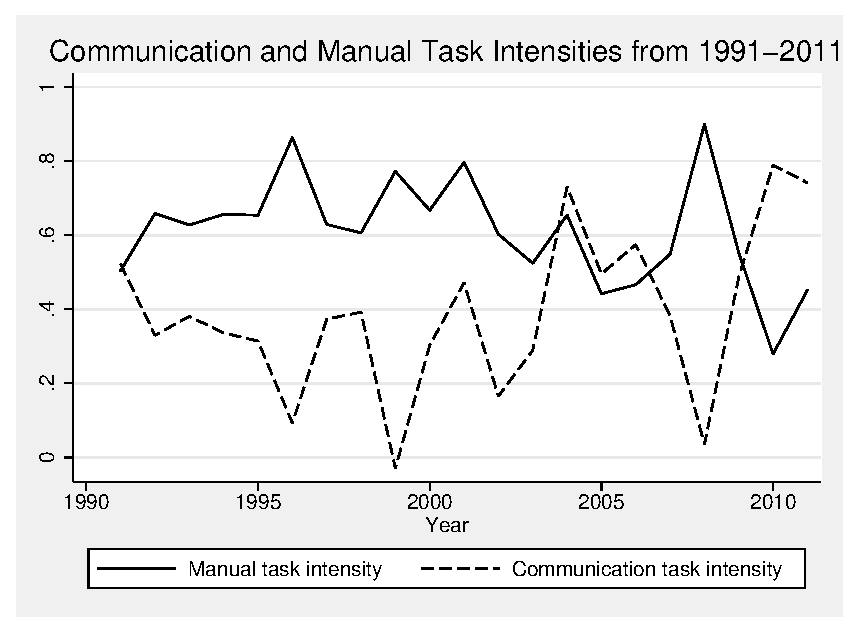
\includegraphics[width=1\textwidth]{data/skillIntensities.eps}
		\caption{Communication and Manual Task Intensities 1991-2011}
		\label{fig:skillIntensity}
	}
	\small
	{\bf Source:} Author's calculations on SAKE data from 1991-2011 and recalculated O*NET abilities by \citet{PeriSparber2009}.\\
	{\bf Notes:} This graph shows the manual and communication task intensities of native born low and medium educated workers within Switzerland evolving over time.
\end{figure}

% 4) little conclusion about my results
As Figure \ref{fig:skillIntensity} suggests through the overall increased communication task intensity, I do find significant effects of immigration on native workers with low and medium education by increasing their absolute and relative supply of communication tasks intensity, suggesting that they indeed are forced to specialise in more communication intensive occupations.\\
The enactment of the Free Movement of Persons Agreement in 2002 led to an increased effect on communication intensity of tasks supplied by the native work force.\\

% 5) thesis structure
I will start giving an overview about related literature and how the skill and task based model was developed in the following section 2. Section 3 will then examine the migration patterns of Switzerland focusing on the two key figures, examining immigrants education and their skills. Section 4 introduces the model of \citet{PeriSparber2009}, which later on will be used to empirically test the hypothesis of task specialisation in Switzerland. After describing the relevant datasets and variables in section 5, I will empirically test the assumptions in section 6 with finally giving a conclusion in section 7.


%%%%%%%%%%%%%%
% LITERATURE REVIEW %
%%%%%%%%%%%%%%
\section{Literature Review}
The effects of immigration on natives is a broadly discussed topic among economists and also politically relevant. 
To understand the importance of workforce specialisation when examining the effects of immigration, I will first give an overview of related literature, how it evolves over time and how economists came up with a skill and task based model, which tries to explain the workforce specialisation. I will then show some results of studies from other countries using the skill-task approach and in the end give some insights, what we would expect from Switzerland.\\

As a first approach many studies examined the effect of immigration on wages with textbook models of competitive labor markets, which led to different and confusing set of results, mainly clustering around zero \citep{FriedbergHund1995}.\\

\citet{Borjas2003} then brought up a differentiated approach of measuring the impact of immigration, by accounting for workers education and work experience, clearing up the confusing array of results from previous studies and leading to consistent results, suggesting that immigration has a negative effect on less-educated native workers. Many studies refer to this model as the skill-cell approach based model.\\

The observation, that in the last decades many highly developed countries experienced an increasing demand for occupations requiring abstract and complex skills together with a decreasing demand in routine and manual ones did not fit into the simple model of education experience cells by \citet{Borjas2003} and led to an increased attention by economists.\\
These tendencies have been documented for the United States by \citet{AcemogluAutor2010} and for the European Union by \citet{GoosManningSalomons2009} and \citet{OeschMenes2010}.\\

As stated by \citet{DAmuriPeri2010} and summarised by \citet{AcemogluAutor2010}, the main research trying to explain these tendencies focused on two possible explanations: Once the effect of technology in terms of information and communication technologies increasing the productivity of abstract-complex occupations and substituting for manual and routine ones, and the effect of trade and off-shoring, which allows the reallocation of simple and manual production processes abroad, while not affecting complex occupations.\\

Those factors probably being the main contributors to the experienced change in specific occupation demands, \citet{DAmuriPeri2010} adds to it the specialisation of the native work force as another dimension producing a shift in the supply of tasks.\\

\citet{DAmuriPeri2010} stated the requirement of differences in relative efficiency of skills supply between the two groups, to explain the pattern of average native workers increasingly specialising in complex and abstract production tasks while foreign born workers mostly staying unchanged or rather move to manual and routine tasks.\\
Native and foreign born workers have different comparative advantages and are therefore imperfect substitutes, which was also brought up by \citet{OttavianoPeri2006} and confirmed by \citet{OttavianoPeri2008}.\\

This approach of workforce specialisation is also based on several studies examining the difference between native and foreign born workers. Their conclusion led to imperfect substitution of native and foreign born workers within groups of similar observable characteristics, as in this case education-age groups. Native workers are assumed to possess comparative advantages in complex-abstract and communication skills while foreign born workers are relatively more advanced in manual tasks. The imperfect substitution therefore promotes native work force specialisation in terms of occupational change, due to comparative advantages in individual skills and performed tasks \citep{ManacordaEtAl2006, OttavianoPeri2008, PeriSparber2009}.\\

% MORE JUICE! explaining why focusing on complex/communication tasks? %
There are several similar studies examining the effects on native work force specialisation. Specialisation for foreign born workers is mostly defined as specialisation in manual and routine tasks, requiring the use of physical skills, whereas native work force specialisation is mostly defined as specialisation in abstract and complex tasks requiring analytical thinking \citep{DAmuriPeri2010}, or in more recent literature communication tasks which require language skills \citep{Peri2009-11}.\\

For the United States \citet{Peri2009-11} using a task based model with communication and manual skill measurements, finds significant evidence, that immigration forces native born workers to specialise in more communication intensive tasks due to their comparative advantage in language skills.\\
% WHAT DO OTHER COUNTRIES EXPERIENCE? %

For European countries \citet{DAmuriPeri2010}, also using a task based framework with complex-abstract and manual skill definitions, provides empirical evidence that immigration forces the native work force to specialise in occupations requiring more complex-abstract tasks.\\

Switzerland currently does not have any studies focusing on the effect of immigration on native work force specialisation but the effects on native wages and other occupational effects are documented.\\

Generally studying the differences of native and foreign born workers \citet{GerfinKaiser2010} shows that these two groups are imperfect substitutes across education and experience groups in Switzerland. This being the condition for native workers to specialise within the group is therefore given and is one key measurement putting Switzerland inline with experiences from other European countries and the US.\\

Several studies focusing on the effect of immigration on native wages in Switzerland led to no or at most minimal effects as for example \citet{Favre2011}, \citet{GerfinKaiser2010}, \citet{Kueng2005} and \cite{Sheldon2001} showed. Therefore the specialisation of native workers could be one reason, why the immense immigration inflow in Switzerland had no large impact on the wages.\\

Regarding occupations \citet{OeschMenes2010} reveals massive occupational upgrading in European countries and extensively so in Switzerland. This is an increasing demand for workers at the top of the occupational hierarchy, among managers and professionals in business and social services. This effect could also be caused by native workers specialising in these occupations.\\

To sum up, occupational upgrading and the imperfect substitution of native and foreign born workers in Switzerland could have favoured native work force specialisation in Switzerland as a relevant tendency, explaining the low effects of immigration on native wages. In the next section I will thoroughly inspect the recent development of migration patterns within Switzerland to further examine the possibility of native specialisation due to immigration.

%%%%%%%%%%%%%%%
% MIGRATION PATTERNS  %
%%%%%%%%%%%%%%%
\section{Migration Patterns in Switzerland}
In this section I will describe the migration patterns in Switzerland, to be able to draw conclusions, how Switzerland could be affected in terms of native work force specialisation due to immigration. Important key figures when examining the effect on specialisation are the share of immigrants and their education as well as the distribution across occupations, which I will be focusing on in the next sub sections.\\

Immigration played an important role in the post-war economic development of Switzerland as the share of foreigners in Switzerland's total population rose from 5\% in 1950 to more than 20\% in recent years \citep{Stalder2010}.\\

\begin{figure}[ht]
	{
	\centering
  		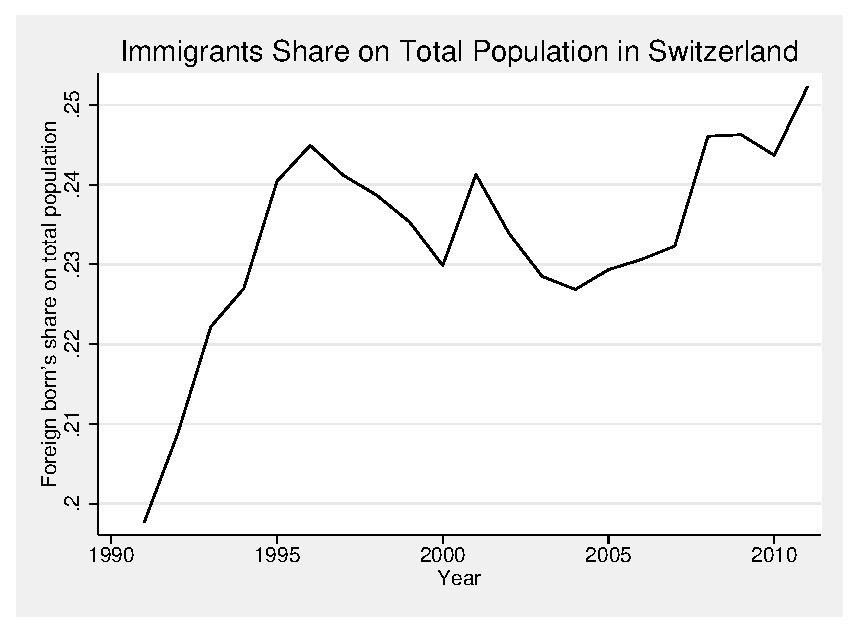
\includegraphics[width=1\textwidth]{data/immigrantsShare.eps}
		\caption{Immigrants Share on Total Population in Switzerland 1991-2011}
		\label{fig:immShare}
	}
	\small
	{\bf Source:} Author's calculations on SAKE data from 1991-2011.\\
	{\bf Notes:} This graph shows the share of foreign born workers within the population of low and medium educated workers in Switzerland evolving over time.
\end{figure}

The migration patterns in Switzerland drastically changed in the last two decades, where the main source countries of immigration shifted from third countries towards EU27 countries due to the Free Movement of Persons Agreement with the European Union.\\

The immigration flow was and still is always closely connected to the cyclical economic development of Switzerland through the labor demand of companies  \citep{SECO2012}. Figure \ref{fig:immShare} shows the close dependency of immigration share with the economic development in Switzerland as after the crisis in 2001 and 2009 the share of immigrants within Switzerland declined.\\

From 1991 to 2001 Switzerland had a mean net migration of +26'400 per year, whereas immigrants from third countries accounted for 26'000 and only 400 from EU27/EFTA countries.\\
This pattern radically changed with the enacting of the Free Movement of Persons Agreement with the European Union in june 2002 after which the net migration drastically increased.
While the yearly mean net migration from EU27/EFTA countries rose to +36'700 from 2002 to 2011, the mean net migration from third countries, stayed nearly unchanged at +25'600 per year \citep{SECO2012}.\\

This increase in net migration and the change of origin countries led to a change in immigrant attainments in terms of education, experience and skills, which I will further examine in the next sub sections.

% IMMIGRATION AND EDUCATION %
\subsection{Immigration and Education}
Regarding education, immigrants are overrepresented at the bottom and the top of the education distribution since 2002 as stated by \citet{Favre2011}, \citet{Stalder2010} and others. \\
Also mentioned by  \citet{SECO2012}, the medium share of immigrants with a tertiary education increased from 38\% in 1994-2002 to 51\% in 2002 - 2010.

\begin{figure}[ht]
	{
	\centering
  		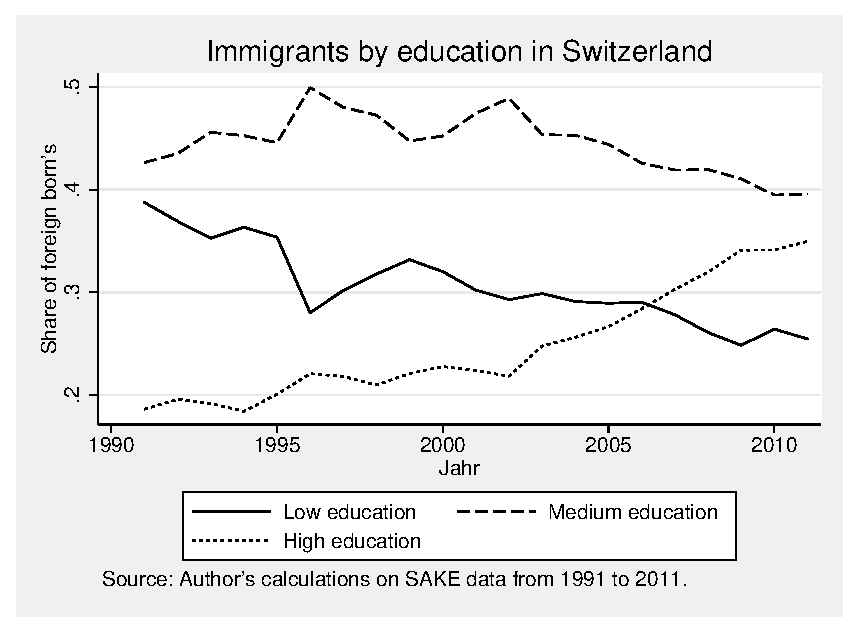
\includegraphics[width=1\textwidth]{data/immigrantsByEducation.eps}
		\caption{Foreign-born share of workers by education groups}
		\label{fig1}
	}
	\small
	{\bf Source:} Author's calculations on SAKE data from 1991-2011.\\
	{\bf Notes:} Each line shows the share of foreign born workers having the specified education on the total number of foreign born workers within Switzerland. I.e. the solid line in 1991 shows that around 38\% of all foreign born workers in Switzerland have a low education. 
\end{figure}

As shown in Figure \ref{fig1}, the share of immigrants in Switzerland with a high education rises since 2002 whereas the share of immigrants with low education declined the last years. Still the share of immigrants with medium education is on a high level.\\


After the Free Movement of Persons Agreement in 2002, occupations performed by highly educated workers experienced the highest percentage change in foreign-borns share, whereas before the agreement occupations with low and middle educated workers had the highest immigrant inflow (Table \ref{table:iscoGroupStats}). \\
Also after the agreement both occupations with high and low educated workers are affected by immigration where before mainly occupations with low and middle educated workers were affected.\\

In recent literature about task specialisation this observation of high skilled foreign born workers inflow is relatively new. It is supposed to behave like \citet{PeriSparber2010} stated for the United States, where highly educated immigrants forced native workers to choose new occupations with less analytical and more communicative content. Therefore looking at task specialisation in terms of manual and communication skills should be an adequate instrument for Switzerland.\\

While many countries still experience mainly low educated immigrant inflows, Switzerland with its increased share of highly educated immigrants suggests a even stronger competition for native workers of all occupation groups because of the comparable education attainment. I will therefore use the communication task intensity of native workers as a key measurement for native workers specialisation, as its communication and language skills are supposed to be one of the main differences between natives and foreign borns.

% IMMIGRATION AND SKILLS %
\subsection{Immigration and Skills}

The foreign born's share in occupations requiring high skills and education steadily rose during the last decades (Figure \ref{figIsco}).\\
During the years from 1991 to 2002, the share of foreign born workers rose in all occupation groups except the professionals and elementary occupation groups. Whereas after 2002 all high and low ranked occupations experienced a higher foreign borns share while the share felt in occupations ranked in the middle like clerks and service workers.\\

\begin{figure}[ht]
	{
		\centering
  		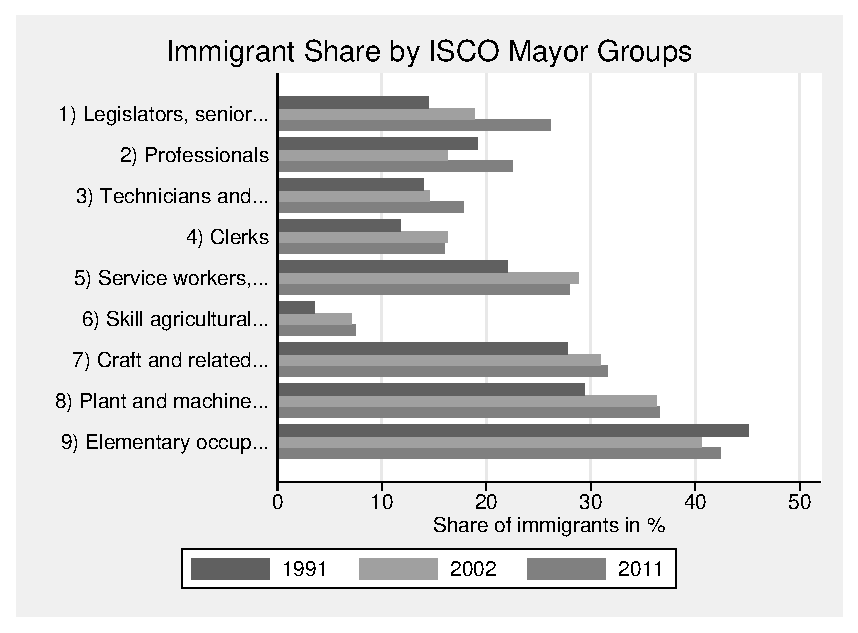
\includegraphics[width=1\textwidth]{data/immigrantsIsco.eps}
		\caption{Foreign-born share of workers by ISCO mayor groups}
		\label{figIsco}
	}
	\small
	{\bf Source:} Author's calculations on SAKE data from 1991, 2002 and 2011.\\
	{\bf Notes:} This graph shows the evolvement of the share of foreign born workers on total population within the ISCO Mayor Groups over time. I.e. in 1991 around 14\% of all workers within the ISCO mayor group "1) Legislators,..." are foreign born. In section \ref{titleData} the ISCO occupation groups are described in detail.
\end{figure}

Figure \ref{figIsco} also reflects the significant increase in high educated immigrants, taking occupations in the upper ISCO mayor groups reflecting the higher skill intensity and therefore the immigrants compete with high skilled native workers which is also shown in Table \ref{table:iscoGroupStats}.\\

This observation is expected, due to the increased share of highly educated immigrants and otherwise inline with observations in other countries experiencing native work force specialisation due to immigration.\\

Figure \ref{figIsco} clearly shows the increased foreign born share throughout all occupation groups. For further analysis these broadly defined mayor groups are too rough. Looking at sub-mayor groups in Table \ref{table:iscoGroupStats}, it is already a little bit refined and the relation between foreign borns share and the communication-manual task intensity ratio can be seen. Therefore native workers gather among occupations with a high communication-manual intensity ratio, signed by the decreasing share of foreign born workers.\\

We can therefore expect, Switzerland to behave similarly to other observations and thus the immigration leading to native work force specialisation in terms of moving to more communication intense tasks.


%%%%%%%%%%
%        MODEL       %
%%%%%%%%%%
\section{The Model}

% PRODUCTION FUNCTION %
\subsection{Production Function}
I will follow the work from \citet{PeriSparber2009} which provides a simple general equilibrium model of comparative advantages in task performance.
I will shortly describe the model on the next pages and then test the key implications of the model in the following sections.\\

Beginning with a constant elasticity of substitution (CES) production function which combines two non-tradable intermediate services, $Y_H$ and $Y_L$ to produce a final tradable good $Y$ in a perfect competitive market with cost minimisation and zero profits.

\begin{equation}\label{eq:1}
	Y=[\beta Y^{\frac{\sigma-1}{\sigma}}_L + (1-\beta)Y_H^{\frac{\sigma-1}{\sigma}}]^{\frac{\sigma}{\sigma-1}}
\end{equation}

Whereas $\sigma \in (0,\infty)$ measures the elasticity of substitution between $Y_H$ and $Y_L$ and $\beta$, $(1-\beta)$ captures their relative productivity.\\
$Y_H$ / $Y_L$ is provided by high/low educated workers ($H$ and $L$) which are defined by workers with secondary education (Matura / Lehre) or less and workers with a tertiary education (university) or more.\\

The model further assumes that in the production of $Y_L$ less-educated workers perform two types of tasks: manual ($M$) and communication ($C$). Manual tasks require the use of physical skills and communication tasks require language skills. Both tasks are combined in a CES function to $Y_L$ with $\theta_L \in (0, \infty)$ measuring their elasticity of substitution and $\beta_L \in (0,1)$ the relative productivity of manual skills.

\begin{equation}\label{eq:2}
	Y_L = [\beta_L M^\frac{\theta_L-1}{\theta_L} + (1-\beta_L)C^\frac{\theta_L-1}{\theta_L}]^\frac{\theta_L}{\theta_L-1}
\end{equation}

Highly educated workers are assumed to only perform analytical tasks that is communication and analytical skills, which are assumed highly substitutable, or are based on the idea that highly educated workers are not affected much by the presence of less educated immigrants, what \citet{PeriSparber2009} showed empirically. Therefore the Production function of highly educated workers is given by $Y_H = H$.

Supposing a competitive labor market and perfect competition, the relative task demand can be expressed by equation (\ref{eq:3}).

\begin{equation}\label{eq:3}
	\frac{C}{M} = (\frac{1-\beta_L}{\beta_L})^{\theta_L}(\frac{w_C}{w_M})^{-\theta_L}
\end{equation}


% RELATIVE SUPPLY OF TASKS %
\subsection{Relative Supply of Tasks}
The wage paid to highly educated workers equals the marginal productivity of $Y_H$ in (\ref{eq:1}): $w_H = P_H$.\\
Allowing heterogeneity between less educated workers in terms of relative task productivity let us account for native / domestic ($L_D$) and foreign born ($L_F$) less educated workers.\\

Each less educated worker provides communication ($\zeta_i$ with $i = \{L_F, L_D\}$) and manual ($\mu_i$) tasks.\\
Further $(\zeta_D/\mu_D) > (\zeta_F/\mu_F)$ is assumed to indicate the comparative advantage in communication tasks for native low educated workers.\\

If a worker has to choose to spend his endowment (time) on to the two different types of tasks, let $l_i$ be the time spent on performing manual tasks and $(1-l_i)$ the time spent on communication tasks. We then have $m_i = (l_i)^\delta\mu_i$ and $c_i = (1-l_i)^\delta\zeta_i$ as the supply of manual and communication task units, with $\delta \in (0,1)$ accounting for decreasing returns form performing a single task to ensure no one will fully specialise.\\

Finally each less educated worker maximises his labor income $w_D$ and $w_F$ respectively, by dividing his endowment into communication and manual tasks, as given by equations (\ref{eq:4}) and (\ref{eq:5}). To account for the difference of foreign born and native workers, foreign borns get a fraction of their marginal productivity $(1-d) \in [0.1]$.

\begin{eqnarray}
	\label{eq:4}
	w_D = (l_D)^\delta \mu_D w_M + (1-l_D)^\delta \zeta_D w_C
	\\
	\label{eq:5}
	w_F = (1-d)(l_F)^\delta \mu_F w_M + (1-l_F)^\delta \zeta_F w_C
\end{eqnarray}

By maximising the wages in respect to $l_i$, the equilibrium relative task supply for each type of worker (D or F) is given by equation (\ref{eq:6}) and the relative time spent on the two type of tasks by equation (\ref{eq:7}).

\begin{eqnarray}
	\label{eq:6}
	\frac{c_i}{m_i} = (\frac{w_C}{w_M})^\frac{\delta}{1-\delta}(\frac{\zeta_i}{\mu_i})^\frac{\delta}{1-\delta}
	\\
	\label{eq:7}
	\frac{l_i}{1-l_i} = (\frac{\zeta_i w_C}{\mu_i w_M})^\frac{1}{\delta-1}
\end{eqnarray}

This model provides a one-to one identifying relationship between relative efficiency in manual/communication tasks ($\zeta_i$,$\mu_i$) and occupational choice of workers of type $i$.\\

As in these simplified model there is no differentiation of abilities within the two types of workers $i$ , $\mu_D$/$\zeta_D$ is the endowment of all native workers and $\mu_F$/$\zeta_F$ the endowment of foreign born workers.\\
Each group will change their occupation if the relative compensation of tasks changes.\\
The product of individual task supply and total labor supply will be the aggregate task supply ($M_i = L_i m_i$ and $C_i = L_i c_i$).\\

Summing the task supply provided by each group will lead to the aggregate relative supply of tasks in the economy described by (\ref{eq:8}) with $\phi(f) = (M_F/(M_F+M_D)) \in (0,1)$ as the share of manual tasks supplied by foreign-born workers given by a simple monotonically increasing transformation of the foreign-born share of less educated workers.

\begin{equation}\label{eq:8}
	\frac{C}{M_D} = \frac{C_F + C_D}{M_F + M_D} = \phi(f)\frac{C_F}{M_F} + (1-\phi(f))\frac{C_D}{M_D}
\end{equation}


With (\ref{eq:6}), (\ref{eq:8}) and equating relative supply and demand the equilibrium relative compensation of tasks is given by (\ref{eq:9}) with the function $\frac{\zeta}{\mu}(f, \frac{\zeta_F}{\mu_F})$ as the weighted average of relative skill endowments among the two worker groups (natives and immigrants), representing an aggregate measure of communication relative to manual ability in the economy. $\frac{\zeta}{\mu}(f, \frac{\zeta_F}{\mu_F})$ depends negatively on $f$ and positively on $\frac{\zeta_F}{\mu_F}$.

\begin{equation}\label{eq:9}
	\frac{w_C^*}{w_M^*} = (\frac{1-\beta_L}{\beta_L})^\frac{(1-\delta)\theta_L}{(1-\delta)\theta_L+\delta}[\frac{\zeta}{\mu}(f, \frac{\zeta_F}{\mu_F})]^\frac{-1}{(1-\delta)\theta_L+\delta}
\end{equation}

By substituting (\ref{eq:9}) into the aggregate relative supply for domestic workers we find the relative provision of tasks equilibrium in (\ref{eq:10}) and the aggregated equilibrium in (\ref{eq:11}).

\begin{equation}\label{eq:10}
	\frac{C_D^*}{M_D^*} = (\frac{1-\beta_L}{\beta_L})^\frac{\delta\theta_L}{(1-\delta)\theta_L+\delta}(\frac{\zeta_D}{\mu_D})^\frac{1}{(1-\delta)}[\frac{\zeta}{\mu}(f, \frac{\zeta_F}{\mu_F})]^{\frac{-1}{(1-\delta)\theta_L+\delta}\frac{\delta}{1-\delta}}
\end{equation}


\begin{equation}\label{eq:11}
	\frac{C^*}{M^*} = (\frac{1-\beta_L}{\beta_L})^\frac{\delta\theta_L}{(1-\delta)\theta_L+\delta}[\frac{\zeta}{\mu}(f, \frac{\zeta_F}{\mu_F})]^\frac{\theta_L}{(1-\delta)\theta_L+\delta}
\end{equation}


% MODEL PREDICTIONS %
\subsection{Model Predictions}
After explaining the model, I will now show how it predicts the impact of immigration on the specialisation of the native work force by their relative supply of communication versus manual tasks.\\

An increasing share of foreign borns in the population affects the model first through relative scarcity of native workers and their communication skills which increases the relative return of communication versus manual tasks, which is shown in equation (\ref{eq:9}).
This affects equation (\ref{eq:10}) through an increased incentive, because of the higher wage return for native workers, to provide more communication tasks, which leads to an increase of the relative supply of communication tasks by natives.\\

Now the equation needs to be standardised, to be able to test it against real world datasets.
This is done by log-linearising the key equilibrium conditions in (\ref{eq:10}). We then obtain equation (\ref{eq:12}) which maps the relative communication intensity provided by native born less-educated workers to the foreign-born share in the population.

\begin{equation}\label{eq:12}
	ln(\frac{C_D}{M_D})_{rt} = \gamma f_{rt} + \alpha^D_r + \tau^D_t + \epsilon^D_{rt}
\end{equation}

Where $\epsilon^D_{rt}$ is the non-correlated zero-mean disturbance term, $\tau^D_t$ the time fixed effects accounting for time-varying technological parameters and $\alpha^D_r$ region fixed effects accounting for variation due to unobserved population characteristics. $\gamma$ represents the key model implications from equation (\ref{eq:12}), $\gamma = -(1/((1-\delta)\theta_L + \delta))(\delta/(1-\delta)) \times (\partial ln(\zeta/\mu)/\partial f)$.\\

The model predicts $\gamma$ to be positive, because in equation (\ref{eq:10}) the foreign-borns share of less-educated workers ($f_{rt}$) within a region causes native workers to increase their relative supply of communication tasks.\\

Therefore accounting for region and year fixed effects a 1 percentage point increase in the share of foreign born workers within the region-year less educated workers is supposed to lead to a $\gamma$ percent increase in relative communication to manual task supply by natives within the same group.


%%%%%%%%%%
%          DATA         %
%%%%%%%%%%
\section{Data and Descriptive Statistics} \label{titleData}
The main dataset used in this thesis is the Swiss Labour Force Survey (SAKE) from 1991 to 2011\footnote{http://www.bfs.admin.ch/bfs/portal/en/index/infothek/erhebungen\_\_quellen/\\
blank/blank/enquete\_suisse\_sur/uebersicht.html}.
It is a yearly household survey conducted for the first time in 1991 and provides information on the structure of the labour force and employment behaviour patterns. It is a telephone survey with around 126'000 interviews per year and therefore because of the small sample size not very accurate on a detailed level but because of the rich information perfectly suitable for aggregated analysis.\\
% Bla bla �ber SAKE fragebogen & datenerfassung %
% dataset: coverage, strength, weaknesses,.. %

For the regression analysis I need data on foreign born's share, canton of living, year of data collection, age, education and individuals occupation.\\

The analysis is restricted to the two periods 1991-2001 and 2002-2011 and only contains individuals in working age from 18 to 64 years old with a positive amount of hours worked and low or medium education.\\
Because of the large increase of highly educated foreign-born workers, I will focus on the low and medium educated population only, as this phenomenon of highly educated immigrant inflow could be handled in a separate study.\\

% what are occupation groups? %
Individuals occupations in Switzerland are coded using the ISCO-88 framework provided by the European Union.
ISCO-88 organises the occupations in a hierarchical framework, with a job at the lowest level as the unit of classification. 
Jobs are grouped to occupations according to the degree of similarity in their constituent tasks and duties. ISCO-88 provides four levels of aggregation. An extensive description and a list of the different levels of occupation grouping is available on their website\footnote{http://www2.warwick.ac.uk/fac/soc/ier/research/links/isco88/}.\\
For our purpose the matching of communication and manual task intensities is done on the lowest ISCO-88 aggregation level on the 4 digit unit groups.\\

The SAKE education variable provides 3 education groups: high school or less, secondary school and tertiary education like university and college. For the analysis I will follow \citet{PeriSparber2009} and focus only on low and middle education groups.\\

Individuals in the SLFS dataset which are identified as foreign born are classified as immigrants.\\

Finally skill measures are supplied by the US Department of Labor's O*NET abilities survey.
The O*NET is a widely used database which describes occupational features including ability measures. Because of its mapping to US job titles, it is mainly used with US census data. Since there are some crosswalks mapping the US job titles to the standardised ISCO-88 occupation codes, there are some recent studies using the O*NET occupation features database because of its rich information also with European datasets \citep{CifuentesEtAl2010}.\\
The O*NET database assigns for each occupation group numerical values to 52 distinct employee abilities. These abilities are used as tasks and skill measures and the provided numbers are recalculated to be comparable across occupations and mapped to the US SOC 1990 codes by  \citet{PeriSparber2009}\footnote{data available on https://www.aeaweb.org/articles.php?doi=10.1257/app.1.3.135}.\\
After the recalculation a value of 0.02 in a specific skill means, that only 2 percent of all workers in the US in 2000 are supplying that specific skill less often.\\
For the analysis some of these skills are grouped together in manual skills containing strength, dexterity, body coordination and flexibility and communication skills containing oral and written expression and comprehension.\\
% why exactly manual and communication skills? %

\begin{figure}[ht]
	{
		\centering
	  	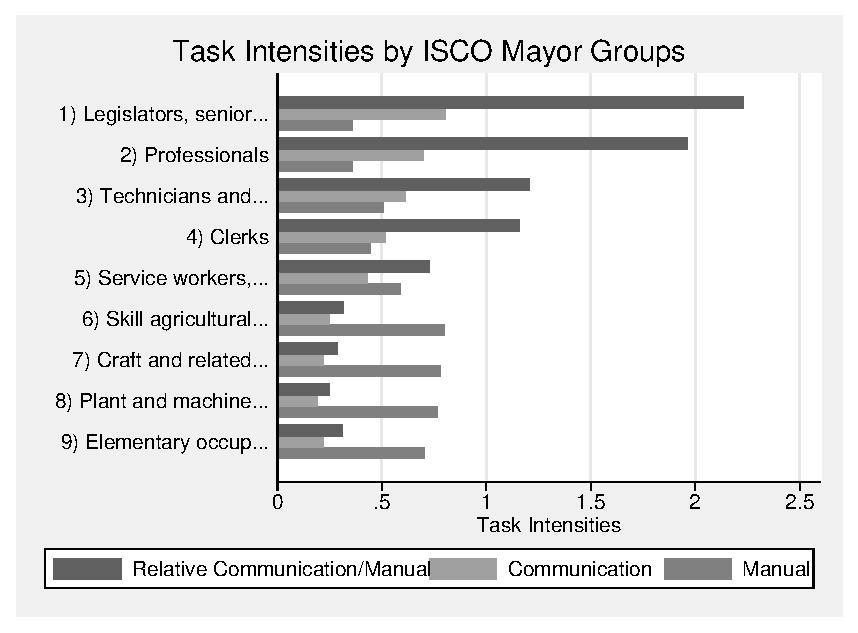
\includegraphics[width=1\textwidth]{data/iscoSkills.eps}
		\caption{Task intensities by ISCO mayor groups}
		\label{figSkill}
	}
	\small
	{\bf Source:} Author's calculations on \citet{PeriSparber2009} abilities dataset being recalculations of the O*NET abilities survey.\\
	{\bf Notes:} This graph shows the relative and absolute task intensities of communication and manual skills within the ISCO mayor groups.
\end{figure}


In the analysis I will build upon these pre calculated variables as measures of communication and manual task intensity of occupations. As this data is mapped to US SOC codes, I will use the crosswalk by Paul Lambert (2003)\footnote{http://www.camsis.stir.ac.uk/occunits/us90toisco88v2.sps} to map US SOC codes to ISCO 88 codes which are provided by the SAKE dataset. 
The abilities dataset uses the detailed US SOC codes which is then mapped to 4 digit ISCO-88 codes.
A full list of occupations mappings can be found in the Appendix Table \ref{table:socToIsco}.\\
% other european countries used onet data and matched to isco codes? %
% explain matching: on what code level do i match? ...%
% what are the underlying assumptions of matching? %


Focusing on ISCO mayor occupation groups the communication-manual task intensities ratio rises with the occupation complexity and skill level. The ratio is highest within legislators, senior officials and managers and lowest within elementary occupations and plant and machine operators and assemblers (Figure \ref{figSkill}).\\
% say why it's relevant for this thesis? %

\begin{table}[ht]
	\centering
	\caption{Descriptive Variable Statistics for the Years 2002-2011}   \label{table:descStat}
	\begin{threeparttable}
\begin{tabular}{lcccccc}
  \toprule
  \midrule
    \multicolumn{6}{c}{1991-2001}\\
    \hline
                            & Mean      & Minimum   & Maximum   & Variance  & Median \\
    \hline
    $f$                     & .2274628  & 0         & .5932468  & .0133737  & .2215283 \\
    $M^D$                   & .6810061  & .3999245  & .970502   & .010743   & .6647032 \\
    $C^D$                   & .3053401  & -.1304807 & .6230747  & .0257592  & .3361611 \\
    $ln(C^D/M^D)$           & -.8414724 & -6.245571 & .3298548  & .7199826  & -.6340535 \\
    $ln(C^D)$               & -1.250581 & -6.512939 & -.4730889 & .5660382  & -1.06055 \\
    $ln(M^D)$               & -.3958475 & -.9164795 & -.0299418 & .023678   & -.4084149 \\

    \hline
    \hline
    \multicolumn{6}{c}{2002-2011}\\
    \hline
                            & Mean      & Minimum   & Maximum   & Variance  & Median \\
    \hline
    $f$                     & .2319105  & .0776128  & .4426769  & .0062502  & .2235558 \\
    $M^D$                   & .5529981  & .2376665  & .9536186   & .0244478   & .5422863 \\
    $C^D$                   & .4574097  & -.0278329 & .8374213  & .0585564  & .4793341 \\
    $ln(C^D/M^D)$           & -.3657868 & -4.775834 & 1.259459  & 1.218147  & -.0822374 \\
    $ln(C^D)$               & -1.009488 & -4.870568 & -.177428 & .7984439  & -.731351 \\
    $ln(M^D)$               & -.6326038 & -1.436887 & -.0474915 & .0832796   & -.6119617 \\
\bottomrule
\end{tabular}
\begin{tablenotes}
  \small
  \item {\bf Source:} Author's calculations on SAKE 1991-2011 data.
  \item {\bf Notes:} Descriptive statistics of all variables used in the regression afterwards. All data variables are collapsed by canton on a yearly basis. $f$ is the foreign born's share within the group, $C^D$, $M^D$ the communication, manual task intensity of native workers respectively and $C^D/M^D$ the relative communication to manual task intensity of native workers within the group.
\end{tablenotes}
\end{threeparttable}
\end{table}

% EXPLAIN how do i aggregate data for regression? %
The individual data is aggregated by Swiss cantons on a yearly basis. Therefore we have eleven years from 1991-2001 and ten years from 2002-2011 with each 26 Swiss cantons.\\
% further explain construction of regions: why? (language => evtl. commuting areas, bigger regions, geographical locations) %
Because of the relative small sample size and small geographical dimensions of the Swiss cantons I will additionally group the aggregated dataset into three broadly defined regions which I will use as dummy variables to control for regional differences.\\
The region variable is constructed with cantons grouped by geographical location which are also broadly connected by their native language (german, italian and french). Therefore I work with three regions where the cantons Waadt, Wallis, Neuenburg, Genf and Jura build the north-western region, the canton Tessin the southern region and all others the north-eastern region. This grouping is also based on the idea that workers will most probably not swap across language barriers.\\

% TODO: HUGE table of descript. stats of used variables (mean, variance,.. variance within regions/cantons,..) %
A descriptive statistic table of all data variables used in this thesis for the regression analysis is shown in Table \ref{table:descStat}.


%%%%%%%%%%%%%%
%  EMPIRICAL RESULTS %
%%%%%%%%%%%%%%
\section{Empirical Results}

This section will empirically test the relationships of foreign born workers share and the native communication and manual task intensities within the medium and low educated population of Switzerland.\\
I will use the empirical specification of equation (\ref{eq:12}) identified by the theoretical model.\\

The regression is done using least squares and weighting each observation by employment in the cell, to account for variations in labor market sizes across cantons. Standard errors are clustered by canton.\\

Additionally I am testing whether immigration has a strong relationship with the average native born workers supply of communication tasks with equation (\ref{eq:communication}) and manual tasks with equation (\ref{eq:manual}).

\begin{eqnarray}
	\label{eq:communication}
	ln(c_D)_{rt}=\alpha_{r}^C + \tau_t^C + \gamma_t^C * f_{rt} + \epsilon^C_{rt}\\
	\label{eq:manual}
	ln(m_D)_{rt}=\alpha_{r}^M + \tau_t^M + \gamma_t^M * f_{rt} + \epsilon^M_{rt}
\end{eqnarray}

\begin{figure}[ht]
	{
		\centering
		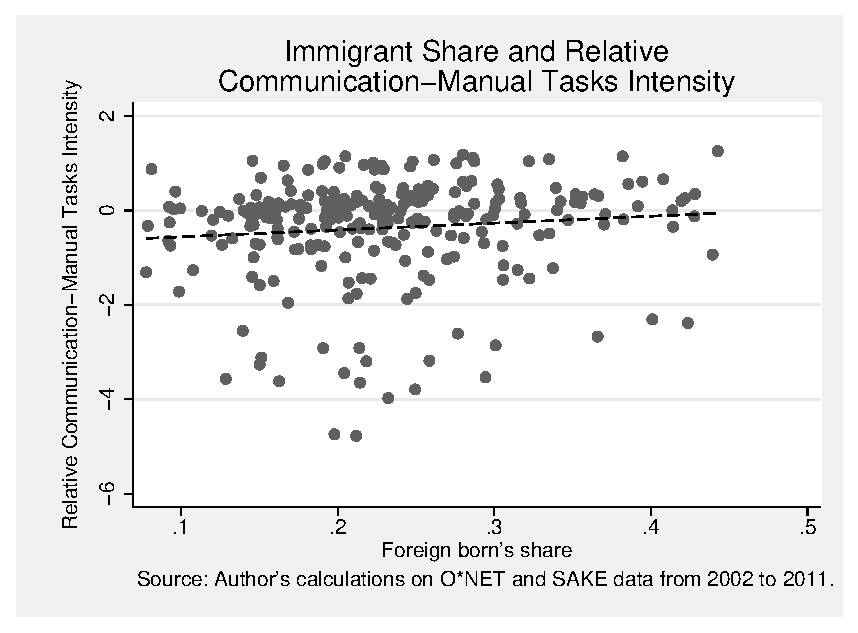
\includegraphics[width=1\textwidth]{data/immigrantsRelativeBasic.eps}
		\caption{Foreign-born share of workers and logarithm of relative communication-manual tasks intensity}
		\label{figRegression}
	}
	\small
	{\bf Source:} Author's calculations on SAKE data from 2002-2011 and recalculated O*NET abilities data from \citet{PeriSparber2009}.\\
	{\bf Notes:} This Graph shows the relationship between the logarithm of relative communication-manual task intensity of native workers and the foreign born's share within low and medium educated workers.
\end{figure}

The regression will use region dummies to account for variations across these broadly specified regions as \citet{PeriSparber2009} did with state dummies on US data, which was not applicable for Swiss data because of the small sample sizes within Swiss cantons and therefore this effect should be caught by the constructed three regions. 
\citet{Borjas2003, Borjas2006}, \citet{Favre2011} and others suggested that effects of immigration could dissipate across the whole country which could be especially true for small scale Switzerland, but \citet{Card2001} and others argue for the use of region dummies and didn't experience any dissipation effects. Therefore I will run the regressions once with and once without region dummies.\\
Additionally including a yearly dummy variable will account for year specific effects.\\

Figure \ref{figRegression} shows the relationship between the logarithm of relative communication-manual task intensity of native workers and the foreign born's share within low and middle educated workers which I am going to estimate.\\

The WLS regression estimates of $\gamma$, $\gamma^C$ and $\gamma^M$ are displayed in Table 1 where the columns (2) and (4) includes region and year dummies and (1) and (3) are limited to year dummies. Column (1) and (2) analysed the period from 1991-2001 while column (3) and (4) analyses the data from 2002-2011. All regressions cluster standard errors on the 26 Swiss cantons.\\
Detailed regression results are listed in the Appendix in Table \ref{table:regWithoutRegions1991} to \ref{table:regWithRegions2002}.\\

\begin{table}[ht]
	{
		\centering
		\caption{Foreign born workers and the native supply of tasks}
		\label{table1}
		  \begin{threeparttable}
     \begin{tabular}{lcccc}
      \toprule
        & \multicolumn{2}{c}{1991-2001} & \multicolumn{2}{c}{2002-2011}\\
        & (1)           & (2)           & (3)           & (4)\\
      \midrule
        $ln(C_D/M_D)_{rt}$  & 1.230177***   & 1.76341***    & 1.568742***   & 2.176916**\\
                            & (0.23)        & (0.36)        & (0.23)        & (0.62)\\
        $ln(c_D)_{rt}$      & 1.013644***   & 1.486272***   & 1.27466***    & 1.777521**\\
                            & (0.22)        & (0.35)        & (0.22)        & (0.58)\\
        $ln(m_D)_{rt}$      & -.2153643***  & -.2777358***  & -.3051352***  & -.4072753***\\
                            & (0.05)        & (0.06)        & (0.03)        & (0.06)\\
        Region dummies      & No            & Yes           & No            & Yes\\
      \bottomrule
    \end{tabular}
  \end{threeparttable}
	}
	\small
	{\bf Source:} Author's calculations on SAKE data from 1991-2011 and recalculated O*NET abilities data from \citet{PeriSparber2009}.\\
      	{\bf Notes:} Dependent Variable: Foreign born's share of workers with medium and low education in the region and year. Regressions are done on a dataset aggregated on a canton and year level.  Each cell contains estimates from a separate regression with standard errors clustered by the 26 Swiss cantons.  Standard errors are reported in parenthesis.
	To construct the average manual $m_D$ and communication $c_D$ skill supply by native workers in a region-year, I first run individual regressions to control for age, gender, experience, and race. The hours-weighted region average of this "cleaned" supply represents the values $c_D$ and $m_D$ and $C_D/M_D$ is their ratio.\\
      	* $p \leq 0.10$ ** $p \leq 0.05$ *** $p \leq 0.01$
\end{table}

All regressions do provide significant results, suggesting that an increased immigration does affect the native work force by increasing their supply of communication tasks and decreasing the manual tasks supply as all estimates of $\gamma$ are significant and positive.\\
Therefore immigration seems to force native workers to specialise in more communication task intensive occupations.\\
Regarding the Region dummies they mostly seem to be insignificant or only significant on a low level and could therefore be omitted or should be replaced by a more accurate measurement as for example commuting regions.\\

Column (1) suggests that a 1 percentage-point increase in the foreign-born share of less and medium educated workers is associated with an 1.23 percent increase in the relative supply of communication-manual tasks within native workers of the same group.
This effect is pretty high compared to results of studies within the United States and should therefore be interpreted carefully and further analysed. The important results nevertheless are the significant positive estimations of $\gamma$ and the significant increase of the estimators after the Free Movement of Persons Agreement in 2002.\\

Comparing the two time periods, before and after the Free Movement of Persons Agreement in 2002, the effect of immigration on communication and manual task intensities of native workers strongly increased and suggests a even stronger specialisation of native workers when affected by immigration since 2002.\\
Therefore the changed immigration patters led to an increase in communication specialisation, a decrease in manual task intensity and a increased relative supply, which could be explained by the increased competition through the increased net migration and also increased demand for managing the new immigrated workers which requires communication skills.\\
The exact source of the increased magnitude of immigration effects could be part of future research efforts.

%%%%%%%%%%%
%  CONCLUSIONS  %
%%%%%%%%%%%
\section{Conclusion}
The Swiss labour market has been significantly affected by immigration during the last decades which led to increasing economic debate about the consequences of immigration. Many of the studies examined the effects of immigration on native wages but did not find large effects. Given the huge immigration inflow and the low wage effects, the model of specialisation of the native workforce could provide an explanation for the low wage effects.\\

In this thesis I will examine the extent of task specialisation of the native work force due to immigration in Switzerland. Using the simple task based model from \citet{PeriSparber2009} as an explanatory framework, this thesis provides new empirical evidence for Switzerland.\\

Using the SAKE data from 1991 to 2011 merged with the O*NET abilities survey to measure the task content of occupations, I find significant results suggesting that, within low and middle educated workers, immigration indeed forces native workers to specialise in occupations with more communication intensive task contents.\\

With the enacting of the Free Movement of Persons Agreement with the European Union in 2002 the magnitude of these effects drastically increased, pushing native workers to even more communication intensive tasks.


%%%%%%%%%%%Bibliography%%%%%%%%%%%
\newpage


\bibliographystyle{agsm}
\bibliography{referenzen}

\newpage

\begin{appendix}
%%%%%%%%%%%Vorlagen%%%%%%%%%%%%%%%%%
\section{Appendix}
\setcounter{table}{0}
\numberwithin{table}{section}

% APPENDIX: table about ISCO mayor groups & TABLE about SOC->ISCO88 matching & TABLE about canton->region matching %

\begin{table}[ht]
	\centering
	\caption{ISCO sub-mayor groups ranked by change in foreign-born's share }
	\label{table:iscoGroupStats}
	\begin{sideways}
  \begin{threeparttable}
     \begin{tabular}{clcccc}
      \toprule
      \midrule

        \multicolumn{6}{c}{1993-2002}\\
        \hline
         &  &  &  & \% of workers in & \\
         & 						& 	       & $C^D/M^D$    & Low \& Middle    & \\
        ISCO & ISCO Sub-Mayor Group Title & $C^D/M^D$ & Rank & Education & $\Delta f/f_{1993}$\\

        \hline
  92 & Agricultural, fishery and related labourers & 0.086 & 21 & 86.36\% & 83.98\% \\
  73 & Precision, handicraft, craft printing and related... & 0.576 & 13 & 92.24\% & 69.732\% \\
  51 & Personal and protective services workers & 0.602 & 12 & 89.93\% & 35.38\% \\

        $\vdots$ &  & $\vdots$ & $\vdots$ & $\vdots$ & $\vdots$ \\

	81 & Stationary plant and related operators & 0.241 & 16 & 91.89\% & -25.86\% \\
	31 & Physical and engineering science associate... & 0.984 & 10 & 71.65\% & -36.87\% \\
	23 & Teaching professionals & 2.193 & 3 & 24.29\% & -39.84\% \\

        \hline
        \hline
        \multicolumn{6}{c}{2002-2011}\\
        \hline
         &  &  &  & \% of workers in & \\
         &            &          & $C^D/M^D$    & Low \& Middle    & \\
        ISCO & ISCO Sub-Mayor Group Title & $C^D/M^D$ & Rank & Education & $\Delta f/f_{2002}$\\
        \hline
  22 & Life science and health professionals & 1.603 & 8 & 4.22\% & 209.63\% \\
	23 & Teaching professionals & 2.182 & 3 & 12.13\% & 138.35\% \\
	31 & Physical and engineering science associate... & 0.955 & 10 & 66.63\% & 59.18\% \\

        $\vdots$ &  & $\vdots$ & $\vdots$ & $\vdots$ & $\vdots$ \\

	11 & Legislators and senior officials & 3.322 & 1 & 35.09\% & -11.39\% \\
	41 & Office clerks & 1.788 & 6 & 82.43\% & -13.55\% \\
	73 & Precision, handicraft, craft printing and related... & 0.640 & 12 & 85.29\% & -15.93\% \\

      \bottomrule
    \end{tabular}
    \begin{tablenotes}
      \small
      \item The 3 highest and 3 lowest  ISCO sub-mayor groups sorted by the percentage change in foreign-borns share in 1993 to 2002 and 2002 to 2011 respectively. $C^D/M^D$ is the relative communication-manual task intensity provided by native born workers.
      \item Relative Communication-Manual task intensity calculations are based on O*NET abilities survey and the foreign born's share and education calculations are based on the SAKE dataset from 1993, 2002 and 2011
    \end{tablenotes}
  \end{threeparttable}
  \end{sideways}
\end{table}


\begin{table}[ht]
	\centering
	\caption{Mapping of US SOC 90 occupation codes to ISCO-88 codes}
	\label{table:socToIsco}
	\begin{threeparttable}
\scalebox{0.42}{
\begin{tabular}{|cc|cc|cc|cc|cc|cc|cc|}
  \toprule
  US SOC 90 & ISCO-88 & US SOC 90 & ISCO-88 & US SOC 90 & ISCO-88 & US SOC 90 & ISCO-88 & US SOC 90 & ISCO-88 & US SOC 90 & ISCO-88 & US SOC 90 & ISCO-88\\
  \midrule
3 & 1110 & 4 & 1120 & 5 & 1120 & 6 & 1120 & 7 & 1231 & 8 & 1232 & 9 & 1233\\
13 & 1233 & 14 & 1229 & 15 & 1229 & 16 & 1226 & 17 & 1315 & 18 & 5121 & 19 & 5143\\
21 & 1310 & 22 & 1310 & 23 & 2411 & 24 & 3412 & 25 & 3410 & 26 & 2149 & 27 & 2412\\
28 & 3416 & 29 & 3416 & 33 & 3416 & 34 & 2419 & 35 & 3151 & 36 & 3444 & 37 & 1229\\
43 & 2141 & 44 & 2145 & 45 & 2147 & 46 & 2147 & 47 & 2146 & 48 & 2146 & 49 & 2145\\
53 & 2142 & 54 & 2213 & 55 & 2143 & 56 & 2149 & 57 & 2145 & 58 & 2145 & 59 & 2149\\
63 & 2148 & 64 & 2131 & 65 & 2121 & 66 & 2121 & 67 & 2122 & 68 & 2121 & 69 & 2111\\
73 & 2113 & 74 & 2112 & 75 & 2114 & 76 & 2110 & 77 & 2213 & 78 & 2211 & 79 & 2213\\
83 & 2221 & 84 & 2221 & 85 & 2222 & 86 & 2223 & 87 & 3224 & 88 & 3226 & 89 & 3229\\
95 & 2230 & 96 & 2224 & 97 & 3223 & 98 & 3226 & 99 & 3226 & 103 & 3226 & 104 & 3229\\
105 & 3226 & 106 & 3221 & 113 & 2310 & 114 & 2310 & 115 & 2310 & 116 & 2310 & 117 & 2310\\
118 & 2310 & 119 & 2310 & 123 & 2310 & 124 & 2310 & 125 & 2310 & 126 & 2310 & 127 & 2310\\
128 & 2310 & 129 & 2310 & 133 & 2310 & 134 & 2310 & 135 & 2310 & 136 & 2310 & 137 & 2310\\
138 & 2310 & 139 & 2310 & 143 & 2310 & 144 & 2310 & 145 & 2310 & 146 & 2310 & 147 & 2321\\
148 & 2321 & 149 & 2322 & 153 & 2310 & 154 & 2310 & 155 & 2332 & 156 & 2331 & 157 & 2321\\
158 & 2340 & 159 & 2359 & 163 & 2412 & 164 & 2432 & 165 & 2431 & 166 & 2441 & 167 & 2445\\
168 & 2442 & 169 & 2442 & 173 & 2141 & 174 & 2446 & 175 & 3460 & 176 & 2460 & 177 & 3480\\
178 & 2421 & 179 & 2422 & 183 & 2451 & 184 & 2451 & 185 & 3471 & 186 & 3473 & 187 & 2455\\
188 & 2452 & 189 & 3131 & 193 & 3473 & 194 & 3470 & 195 & 2451 & 197 & 2419 & 198 & 3472\\
199 & 3475 & 203 & 3211 & 204 & 3225 & 205 & 2432 & 206 & 3133 & 207 & 3231 & 208 & 3211\\
213 & 3113 & 214 & 3119 & 215 & 3115 & 216 & 3119 & 217 & 3118 & 218 & 3118 & 223 & 3211\\
224 & 3111 & 225 & 3111 & 226 & 3143 & 227 & 3144 & 228 & 3132 & 229 & 2132 & 233 & 3123\\
234 & 2421 & 235 & 3100 & 243 & 1314 & 253 & 3412 & 254 & 3413 & 255 & 3411 & 256 & 3429\\
257 & 3429 & 258 & 3415 & 259 & 3415 & 263 & 5220 & 264 & 5220 & 265 & 5220 & 266 & 5220\\
267 & 5220 & 268 & 5220 & 269 & 5220 & 274 & 5220 & 275 & 5220 & 276 & 4211 & 277 & 9110\\
278 & 9112 & 283 & 5210 & 284 & 3417 & 285 & 5200 & 303 & 1240 & 304 & 1240 & 305 & 1231\\
306 & 4223 & 307 & 4133 & 308 & 3122 & 309 & 3122 & 313 & 4115 & 314 & 4111 & 315 & 4111\\
316 & 4190 & 317 & 4222 & 318 & 4221 & 319 & 4222 & 323 & 4222 & 325 & 4190 & 326 & 4100\\
327 & 4132 & 328 & 4121 & 329 & 4141 & 335 & 4141 & 336 & 4190 & 337 & 4121 & 338 & 4121\\
339 & 4121 & 343 & 4121 & 344 & 4114 & 345 & 4190 & 346 & 4142 & 347 & 4114 & 348 & 4223\\
353 & 3132 & 354 & 4142 & 355 & 4142 & 356 & 4212 & 357 & 9151 & 359 & 4133 & 363 & 4132\\
364 & 4131 & 365 & 4131 & 366 & 9153 & 368 & 4131 & 373 & 4133 & 374 & 4132 & 375 & 3417\\
376 & 3417 & 377 & 3443 & 378 & 4215 & 379 & 4100 & 383 & 4212 & 384 & 4143 & 385 & 4113\\
386 & 4122 & 387 & 3310 & 389 & 4190 & 403 & 8264 & 404 & 5122 & 405 & 5121 & 406 & 5131\\
407 & 9132 & 413 & 5161 & 414 & 5162 & 415 & 9152 & 416 & 5161 & 417 & 5161 & 418 & 5162\\
423 & 5162 & 424 & 5163 & 425 & 8312 & 426 & 5169 & 427 & 5169 & 433 & 5121 & 434 & 5123\\
435 & 5123 & 436 & 5122 & 438 & 5123 & 439 & 9132 & 443 & 5123 & 444 & 5120 & 445 & 3225\\
446 & 3221 & 447 & 5132 & 448 & 9141 & 449 & 9131 & 453 & 9140 & 454 & 9151 & 455 & 7143\\
456 & 5141 & 457 & 5141 & 458 & 5141 & 459 & 9152 & 461 & 5113 & 462 & 9152 & 463 & 9152\\
464 & 9151 & 465 & 3460 & 466 & 5131 & 467 & 3320 & 468 & 5131 & 469 & 5100 & 473 & 6133\\
474 & 6113 & 475 & 1311 & 476 & 1311 & 477 & 6132 & 479 & 9211 & 483 & 6151 & 484 & 9211\\
485 & 6132 & 486 & 9211 & 487 & 9211 & 488 & 7415 & 489 & 3152 & 494 & 6141 & 495 & 9142\\
496 & 6141 & 497 & 3142 & 498 & 6150 & 499 & 6154 & 503 & 7230 & 505 & 7231 & 506 & 7231\\
507 & 7231 & 508 & 7232 & 509 & 7230 & 514 & 7213 & 515 & 7232 & 516 & 7233 & 517 & 7233\\
518 & 7233 & 519 & 7233 & 523 & 7242 & 525 & 7242 & 526 & 7241 & 527 & 7245 & 529 & 7244\\
533 & 7241 & 534 & 7241 & 535 & 7310 & 536 & 7222 & 538 & 7242 & 539 & 7233 & 543 & 7233\\
544 & 7233 & 547 & 7230 & 549 & 7230 & 553 & 7122 & 554 & 7124 & 555 & 7240 & 556 & 7141\\
557 & 7136 & 558 & 7510 & 563 & 7122 & 564 & 7122 & 565 & 7132 & 566 & 7132 & 567 & 7132\\
569 & 7124 & 573 & 7129 & 575 & 7137 & 576 & 7137 & 577 & 7245 & 579 & 7141 & 583 & 7141\\
584 & 7133 & 585 & 7136 & 587 & 7136 & 588 & 7123 & 589 & 7135 & 593 & 7134 & 594 & 8332\\
595 & 7131 & 596 & 7213 & 597 & 7214 & 598 & 8113 & 599 & 7129 & 613 & 7110 & 614 & 8113\\
615 & 7112 & 616 & 8111 & 617 & 7111 & 628 & 7510 & 634 & 7222 & 635 & 7222 & 636 & 7311\\
637 & 7222 & 639 & 7223 & 643 & 7213 & 644 & 7224 & 645 & 7222 & 646 & 7222 & 647 & 7313\\
649 & 7343 & 653 & 7213 & 654 & 7213 & 655 & 7213 & 656 & 7422 & 657 & 7422 & 658 & 7422\\
659 & 7420 & 666 & 7433 & 667 & 7433 & 668 & 7437 & 669 & 7442 & 674 & 7436 & 675 & 7310\\
676 & 7310 & 677 & 7322 & 678 & 7311 & 679 & 7345 & 683 & 8282 & 684 & 7310 & 686 & 7411\\
687 & 7412 & 688 & 8270 & 689 & 9321 & 693 & 7331 & 694 & 8163 & 695 & 8161 & 696 & 8160\\
699 & 8160 & 703 & 7223 & 704 & 8211 & 705 & 8211 & 706 & 8211 & 707 & 8122 & 708 & 8211\\
709 & 8223 & 713 & 7221 & 714 & 7223 & 715 & 8211 & 717 & 8400 & 719 & 8122 & 723 & 8223\\
724 & 8123 & 725 & 8290 & 726 & 8141 & 727 & 8141 & 728 & 8240 & 729 & 8240 & 733 & 8141\\
734 & 8251 & 735 & 7344 & 736 & 7341 & 737 & 8251 & 738 & 8261 & 739 & 8262 & 743 & 8269\\
744 & 8263 & 745 & 8266 & 747 & 8264 & 748 & 8264 & 749 & 8269 & 753 & 8229 & 754 & 8290\\
755 & 8229 & 756 & 8151 & 757 & 8154 & 758 & 8290 & 759 & 7142 & 763 & 8274 & 764 & 8275\\
765 & 8290 & 766 & 8131 & 768 & 8151 & 769 & 8290 & 773 & 3132 & 774 & 8251 & 777 & 8290\\
779 & 8290 & 783 & 7212 & 784 & 7212 & 785 & 8290 & 786 & 7520 & 787 & 7520 & 789 & 7141\\
793 & 7323 & 795 & 7520 & 796 & 8290 & 797 & 8290 & 798 & 8290 & 799 & 8290 & 803 & 4133\\
804 & 8324 & 806 & 8322 & 808 & 8323 & 809 & 8322 & 813 & 9152 & 814 & 9333 & 823 & 5112\\
824 & 8311 & 825 & 8312 & 826 & 8310 & 828 & 8340 & 829 & 8340 & 833 & 3141 & 834 & 8340\\
843 & 7520 & 844 & 8330 & 845 & 8333 & 848 & 8333 & 849 & 8333 & 853 & 8332 & 855 & 8332\\
856 & 8334 & 859 & 8330 & 864 & 7510 & 865 & 7234 & 866 & 9313 & 867 & 9313 & 868 & 9311\\
869 & 9313 & 874 & 9320 & 875 & 9161 & 876 & 9333 & 877 & 9333 & 878 & 9321 & 883 & 9333\\
885 & 7234 & 887 & 9142 & 888 & 9322 & 889 & 9300 & 903 & 110 & 904 & 110 & 905 & 110\\
\bottomrule
\end{tabular}
}
\begin{tablenotes}
  \small
  \item {\bf Source:} Paul Lambert (2003) (http://www.camsis.stir.ac.uk/occunits/us90toisco88v2.sps)
  \item {\bf Notes:} Mapping of US SOC 90 occupation codes to ISCO-88 four digit codes.
\end{tablenotes}
\end{threeparttable}
\end{table}


\begin{table}[ht]
	{
		\centering
		\caption{Foreign Born Workers and the Native Supply of Tasks without region dummies 1991-2001}
		\label{table:regWithoutRegions1991}
		1991-2000 Foreign Born Workers and the Native Supply of Tasks
            &   Relative2   &   Language2   &     Manual2   \\
            &        b/se   &        b/se   &        b/se   \\
share_fb    &    1.230177***&    1.013644***&   -.2153643***\\
            &      (0.23)   &      (0.22)   &      (0.05)   \\
y2          &   -.7448036***&   -.4742726***&    .2705156***\\
            &      (0.03)   &      (0.02)   &      (0.01)   \\
y3          &   -.5668497***&   -.3433491***&    .2234694***\\
            &      (0.03)   &      (0.02)   &      (0.01)   \\
y4          &   -.7410498***&   -.4716138***&    .2693986***\\
            &      (0.02)   &      (0.02)   &      (0.01)   \\
y5          &   -.8204196***&   -.5519433***&    .2684247***\\
            &      (0.03)   &      (0.03)   &      (0.01)   \\
y6          &   -2.410448***&   -1.861747***&     .548895***\\
            &      (0.12)   &      (0.12)   &      (0.01)   \\
y7          &   -.6118011***&   -.3811955***&    .2305545***\\
            &      (0.04)   &      (0.03)   &      (0.01)   \\
y8          &   -.5287092***&   -.3342823***&    .1943723***\\
            &      (0.03)   &      (0.02)   &      (0.01)   \\
y9          &   -4.881031***&   -4.458661***&    .4349388***\\
            &      (0.90)   &      (0.89)   &      (0.01)   \\
y10         &   -.8700706***&   -.5826167***&    .2874122***\\
            &      (0.03)   &      (0.03)   &      (0.01)   \\
y11         &   -.6188269***&   -.1511142***&    .4676564***\\
            &      (0.02)   &      (0.02)   &      (0.01)   \\
_cons       &   -.2199054***&   -.8621325***&   -.6424731***\\
            &      (0.05)   &      (0.05)   &      (0.01)   \\
r2          &    .8795232   &    .8634068   &    .9396622   \\
N           &         266   &         266   &         288   \\
vce         &     cluster   &     cluster   &     cluster   \\

	}
	\small
	{\bf Source:} Author's calculations on SAKE 1991-2001 and recalculated O*NET abilities data from \citet{PeriSparber2009}.\\
	{\bf Note:} Fixed effects regressions clustered by cantons. Standard errors are reported in parenthesis. $f$ is the foreign born's share of workers with medium and low education within the year canton cell and y* the yearly dummies for 1991-2001.\\
      	* $p \leq 0.10$ ** $p \leq 0.05$ *** $p \leq 0.01$
\end{table}


\begin{table}[ht]
	{
		\centering
		\caption{Foreign Born Workers and the Native Supply of Tasks with region dummies 1991-2001}
		\label{table:regWithRegions1991}
		1991-2000 Foreign Born Workers and the Native Supply of Tasks with Canton Dummies
            &    Relative   &    Language   &      Manual   \\
            &        b/se   &        b/se   &        b/se   \\
share_fb    &     1.76341***&    1.486272***&   -.2777358***\\
            &      (0.36)   &      (0.35)   &      (0.06)   \\
st2         &   -.1490664*  &   -.1300607*  &    .0172462   \\
            &      (0.06)   &      (0.06)   &      (0.02)   \\
st3         &   -.1878766***&   -.1670845***&    .0214546   \\
            &      (0.04)   &      (0.04)   &      (0.02)   \\
y2          &   -.7536568***&   -.4821116***&    .2715473***\\
            &      (0.03)   &      (0.02)   &      (0.01)   \\
y3          &    -.578631***&   -.3537928***&    .2248535***\\
            &      (0.03)   &      (0.03)   &      (0.01)   \\
y4          &   -.7560814***&   -.4849425***&    .2711615***\\
            &      (0.03)   &      (0.03)   &      (0.01)   \\
y5          &   -.8420514***&   -.5711073***&    .2709605***\\
            &      (0.03)   &      (0.03)   &      (0.01)   \\
y6          &   -2.436067***&   -1.884452***&    .5518863***\\
            &      (0.12)   &      (0.12)   &      (0.01)   \\
y7          &   -.6323718***&    -.399428***&    .2329675***\\
            &      (0.04)   &      (0.04)   &      (0.01)   \\
y8          &   -.5502623***&   -.3533803***&    .1969022***\\
            &      (0.04)   &      (0.03)   &      (0.01)   \\
y9          &   -4.861874***&   -4.441271***&    .4371318***\\
            &      (0.88)   &      (0.87)   &      (0.01)   \\
y10         &   -.8863363***&   -.5970411***&    .2893211***\\
            &      (0.04)   &      (0.03)   &      (0.01)   \\
y11         &   -.6415377***&   -.1712493***&    .4703199***\\
            &      (0.03)   &      (0.03)   &      (0.01)   \\
_cons       &   -.2881851***&    -.922625***&   -.6343739***\\
            &      (0.07)   &      (0.07)   &      (0.01)   \\
r2          &    .8848349   &    .8686237   &    .9418497   \\
N           &         266   &         266   &         288   \\
vce         &     cluster   &     cluster   &     cluster   \\

	}
	\small
	{\bf Source:} Author's calculations on SAKE 1991-2001 and recalculated O*NET abilities data from \citet{PeriSparber2009}.\\
	{\bf Note:} Fixed effects regressions clustered by cantons. Standard errors are reported in parenthesis. $f$ is the foreign born's share of workers with medium and low education within the year canton cell, r* are the region dummies and y* the yearly dummies for 1991-2001.\\
      	* $p \leq 0.10$ ** $p \leq 0.05$ *** $p \leq 0.01$
\end{table}

\begin{table}[ht]
	{
		\centering
		\caption{Foreign Born Workers and the Native Supply of Tasks without region dummies 2002-2011}
		\label{table:regWithoutRegions2002}
		Foreign Born Workers and the Native Supply of Tasks
            &   Relative2   &   Language2   &     Manual2   \\
            &        b/se   &        b/se   &        b/se   \\
share_fb    &    1.568058***&    1.123055***&   -.4444496***\\
            &      (0.20)   &      (0.14)   &      (0.06)   \\
y2          &     .718114***&    .5752517***&   -.1428594***\\
            &      (0.03)   &      (0.03)   &      (0.00)   \\
y3          &    1.430272***&    1.508669***&    .0784019***\\
            &      (0.05)   &      (0.04)   &      (0.00)   \\
y4          &    1.428882***&    1.114975***&   -.3139052***\\
            &      (0.04)   &      (0.04)   &      (0.01)   \\
y5          &    1.522414***&    1.263016***&   -.2593962***\\
            &      (0.04)   &      (0.04)   &      (0.01)   \\
y6          &    .9462709***&     .851276***&   -.0949944***\\
            &      (0.04)   &      (0.04)   &      (0.01)   \\
y7          &   -1.884076***&   -1.480692***&     .407877***\\
            &      (0.14)   &      (0.14)   &      (0.01)   \\
y8          &    1.154218***&    1.075234***&   -.0789913***\\
            &      (0.04)   &      (0.04)   &      (0.00)   \\
y9          &    2.330952***&    1.562207***&   -.7687515***\\
            &      (0.04)   &      (0.05)   &      (0.01)   \\
y10         &    1.771854***&    1.491115***&   -.2807501***\\
            &      (0.04)   &      (0.04)   &      (0.01)   \\
_cons       &   -1.688526***&   -2.088886***&   -.4004975***\\
            &      (0.07)   &      (0.06)   &      (0.01)   \\
r2          &    .9652424   &     .952649   &    .9795228   \\
N           &         255   &         255   &         260   \\
vce         &     cluster   &     cluster   &     cluster   \\

	}
	\small
	{\bf Source:} Author's calculations on SAKE 2002-2011 and recalculated O*NET abilities data from \citet{PeriSparber2009}.\\
	{\bf Note:} Fixed effects regressions clustered by cantons. Standard errors are reported in parenthesis. $f$ is the foreign born's share of workers with medium and low education within the year canton cell and y* the yearly dummies for 2002-2011.\\
      	* $p \leq 0.10$ ** $p \leq 0.05$ *** $p \leq 0.01$
\end{table}


\begin{table}[ht]
	{
		\centering
		\caption{Foreign Born Workers and the Native Supply of Tasks with region dummies 2002-2011}
		\label{table:regWithRegions2002}
		Foreign Born Workers and the Native Supply of Tasks with Canton Dummies
            &    Relative   &    Language   &      Manual   \\
            &        b/se   &        b/se   &        b/se   \\
share_fb    &     2.11851***&    1.425475***&   -.6826757***\\
            &      (0.36)   &      (0.26)   &      (0.10)   \\
st2         &    -.066633   &   -.0270345   &     .038112*  \\
            &      (0.06)   &      (0.04)   &      (0.02)   \\
st3         &   -.1577254*  &   -.0877796   &    .0676354** \\
            &      (0.07)   &      (0.05)   &      (0.02)   \\
y2          &    .7211133***&    .5768925***&   -.1441644***\\
            &      (0.03)   &      (0.03)   &      (0.01)   \\
y3          &    1.435137***&    1.511349***&    .0763026***\\
            &      (0.04)   &      (0.04)   &      (0.01)   \\
y4          &      1.4314***&    1.116371***&   -.3149828***\\
            &      (0.04)   &      (0.04)   &      (0.01)   \\
y5          &     1.52464***&    1.264247***&   -.2603527***\\
            &      (0.04)   &      (0.04)   &      (0.01)   \\
y6          &    .9468043***&    .8515807***&   -.0952145***\\
            &      (0.04)   &      (0.04)   &      (0.01)   \\
y7          &   -1.893225***&   -1.485793***&    .4108233***\\
            &      (0.13)   &      (0.14)   &      (0.01)   \\
y8          &    1.146508***&    1.070996***&   -.0756587***\\
            &      (0.04)   &      (0.04)   &      (0.01)   \\
y9          &    2.324457***&    1.558641***&   -.7659391***\\
            &      (0.04)   &      (0.05)   &      (0.01)   \\
y10         &    1.760482***&    1.484872***&   -.2758228***\\
            &      (0.05)   &      (0.05)   &      (0.01)   \\
_cons       &   -1.788861***&   -2.144136***&   -.3572937***\\
            &      (0.07)   &      (0.05)   &      (0.02)   \\
r2          &    .9673018   &    .9536579   &    .9848818   \\
N           &         255   &         255   &         260   \\
vce         &     cluster   &     cluster   &     cluster   \\

	}
	\small
	{\bf Source:} Author's calculations on SAKE 2002-2011 and recalculated O*NET abilities data from \citet{PeriSparber2009}.\\
	{\bf Note:} Fixed effects regressions clustered by cantons. Standard errors are reported in parenthesis. $f$ is the foreign born's share of workers with medium and low education within the year canton cell, r* are the region dummies and y* the yearly dummies for 2002-2011.\\
      	* $p \leq 0.10$ ** $p \leq 0.05$ *** $p \leq 0.01$
\end{table}


\end{appendix}

\end{document}